\section{Mesoscale Eddies}\label{sec:mesoscale}

\subsection{Evaluation of Detection Results}\label{sec:mesoscale-detections}

The detection algorithm of \textcite{faghmous-2015} detects $\around \SI{25}{\percent}$ more eddies in \ac{hr} than in \ac{mr}. During the three years of analysis, $\num[separate-uncertainty]{24.9(2)}$ cyclones and $\num[separate-uncertainty]{22.2(2)}$ anticyclones are detected in \ac{mr} per day. On the other hand, $\num[separate-uncertainty]{34.5(3)}$ cyclones and $\num[separate-uncertainty]{29.7(2)}$ anticyclones are detected in \ac{hr} per day. Both models show a slight increase in the number of detected eddies from March to October, but the ratio of cyclones to anticyclones is constant in the course of the year ($\num[separate-uncertainty]{1.14(1)}$ in \ac{mr}, $\num[separate-uncertainty]{1.18(1)}$ in \ac{hr}). The ratio compares very well to ratios of $1.18$ reported by \textcite[see their Figure 5]{kurian-2011-eddy-props} and $1.15 - 1.25$ reported by \textcite{nagai-2015-dom-role-meso}, albeit they used a different detection algorithm. The number of detections is not directly comparable because the studies analysed a larger part of the \ac{ccs}.\\
\\
The increased number of detections in \ac{hr} is caused by detection of more smaller eddies with a radius $r_e \le \SI{30}{\kilo\metre}$. This can be seen in the distribution of $r_e$ which is shown in \autoref{fig:eddy-area}. Only $\SI[separate-uncertainty]{37.0(12)}{\percent}$ of all detected eddies in \ac{mr} have a radius $r_e \le \SI{30}{\kilo\metre}$, whereas $\SI[separate-uncertainty]{59.5(16)}{\percent}$ in \ac{hr} fall in this category. For the range $\SI{30}{\kilo\metre} \le r_e <  \SI{100}{\kilo\metre}$, the number of detections is very similar in \ac{mr} and \ac{hr}. Very large eddies with radius $r_e > \SI{100}{\kilo\metre}$ are less present in \ac{hr} but are rare in both models. The number of detections decreases exponentially with increasing radius which is consistent with results from \textcite[see their Figure 5]{kurian-2011-eddy-props}.\\
The detection algorithm defines eddies as closed contours in \ac{ssh} around a single extremum \autocite{faghmous-2015}. Hence, the algorithm is sensitive to the smoothness of the \ac{ssh} field and thus to the horizontal resolution. To evaluate the impact of this effect, the \ac{ssh} field of \ac{hr} was interpolated to the grid of \ac{mr}. As expected, the fraction of smaller eddies is reduced to $\SI[separate-uncertainty]{42.6(10)}{\percent}$, but it is still higher than for \ac{mr}. This indicates that there are indeed more smaller eddies in \ac{hr} than in \ac{mr} and that it is not just caused by the sensitivity of the detection algorithm.\\
\begin{figure}
    \centering
    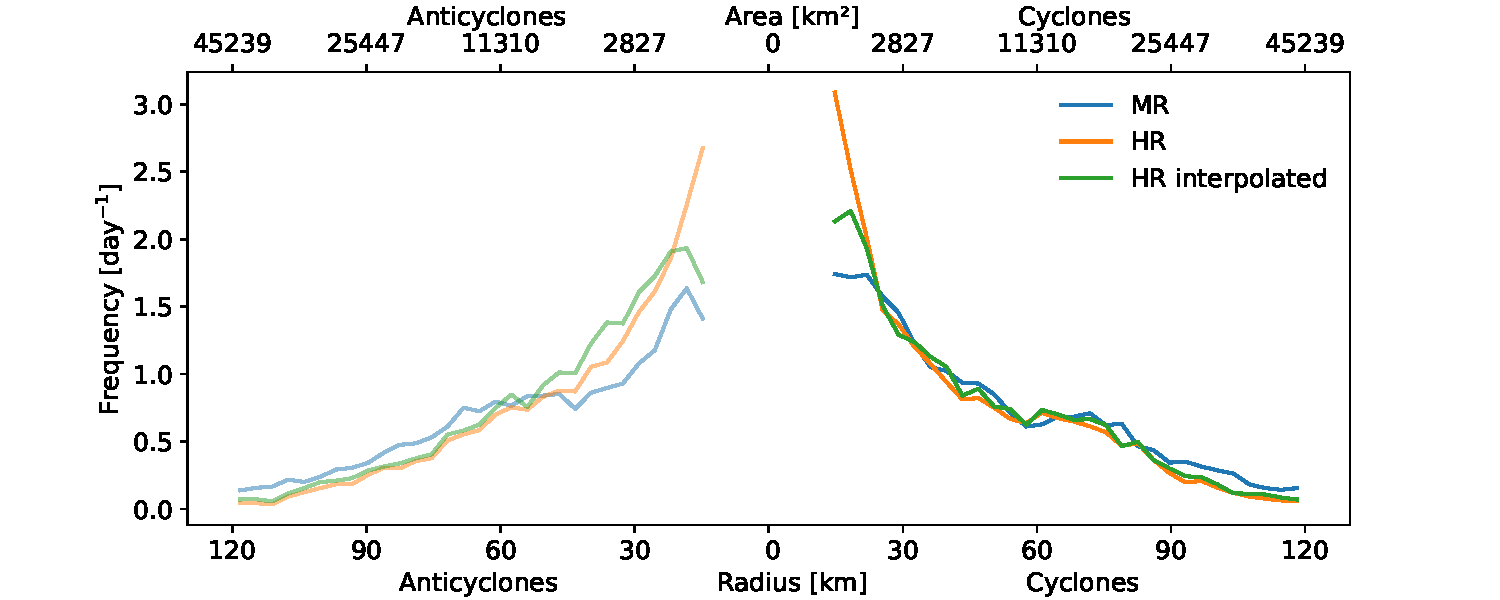
\includegraphics[width=15cm]{../figures/result_eddies_area.pdf}
    \caption[Distribution of eddy radius]{\textbf{Distribution of eddy radius}. The distribution is plotted to the right for cyclones and to the left for anticyclones.}\label{fig:eddy-area}
\end{figure}
\\
The radius of eddies increases with their distance to the coast (see \autoref{fig:meso_d2c}). Within the first $\SI{250}{\kilo\metre}$ off the coast, the average radius increases by $\around \SI{60}{\percent}$ from $\SI{19}{\kilo\metre}$ ($\SI{13}{\kilo\metre}$) to $\SI{48}{\kilo\metre}$ ($\SI{31}{\kilo\metre}$) in \ac{mr} (\ac{hr}). Beyond $\SI{250}{\kilo\metre}$, eddies grow slower and approach a radius of $\SI{63}{\kilo\metre}$ ($\SI{48}{\kilo\metre}$) around $\SI{800}{\kilo\metre}$ off the coast in \ac{mr} (\ac{hr}). This evolution has also been observed by \textcite[see their Figure 8]{kurian-2011-eddy-props}.\\
\\
Regarding the lifetime, cyclones are more stable than anticyclones, especially in \ac{hr}. On the one hand, the average lifetime of cyclones ($\SI{83}{\day}$ in \ac{mr}, $\SI{58}{\day}$ in \ac{hr}) is longer than the average lifetime of anticyclones ($\SI{70}{\day}$ in \ac{mr}, $\SI{49}{\day}$ in \ac{hr}). Though, the values have high variance of $\around \SI{150}{\percent}$ as the lifetimes can reach from few days to several months. On the other hand, cyclonic dominance increases for long-lived eddies. More precisely, the ratio of cyclonic to anticyclonic tracks increases with an increasing threshold of minimum lifetime (see \autoref{fig:meso_lft}). This is in accordance with results of \textcite[see their Figure 5]{kurian-2011-eddy-props}. The effect is stronger in \ac{hr} as the ratio is larger in \ac{hr} for every minimum lifetime threshold. For a minimum lifetime of $\SI{90}{\day}$ for example, there are 113 (115) cyclones and only 95 (83) anticyclones in \ac{mr} (\ac{hr}). Results regarding lifetime of eddies should be treated with caution, because the tracks are likely to be biased to short tracks. The reason is that missing detections or eddy interactions can lead to an early stopping of tracks and eventually a starting of new tracks. Nevertheless, a comparison of cyclones and anticyclones is valid as both are affected by this issue.
\begin{figure}[h]
    \centering
    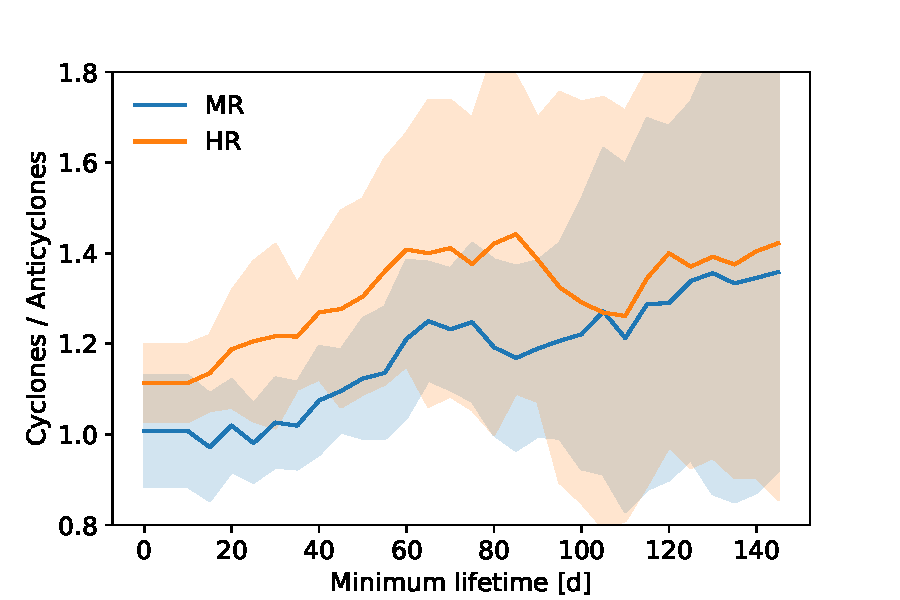
\includegraphics[width=10cm]{figures/result_eddies_lft_tracks.pdf}
    \caption[Ratio of cyclonic to anticyclonic tracks]{\textbf{Ratio of cyclonic to anticyclonic tracks}. The shaded area represents the interannual variability. The reason for the high variability is twofold: the number of tracks decreases with increasing threshold and the tracks had to be attributed to a single year although they can span two years.}
    \label{fig:meso_lft}
\end{figure}

\subsection{Seasonality of Eddy Strength}\label{sec:mesoscale-comparison}

The most energetic mesoscale eddies are formed nearshore during summer. This can be seen in \autoref{fig:eddy-eke} which shows the \ac{eke} associated with cyclones and anticyclones. During summer and autumn, the eddies move offshore (westwards) and reach the offshore region in winter where most of the associated energy dissipates. This seasonality has been observed in various other studies as well \autocite{kelly-1998-eke-obs, checkley-2009-currentstructure-calcs, chaigneau-2009-four-major-ebus, kurian-2011-eddy-props}. Compared to \ac{mr}, the overall \ac{eke} (i.e. independent of eddy detections) increases by $\SI{10.2(5)}{\percent}$ in \ac{hr} with a maximum increase of $\SI{14.9(10)}{\percent}$ during spring. This matches well to observations of \textcite{schubert-2020-subm-energy-cascade} who observed a reduction of kinetic energy in the mesoscale by $\around \SI{20}{\percent}$ when submesoscale motions are not resolved.\\
\begin{sidewaysfigure}
    \centering
    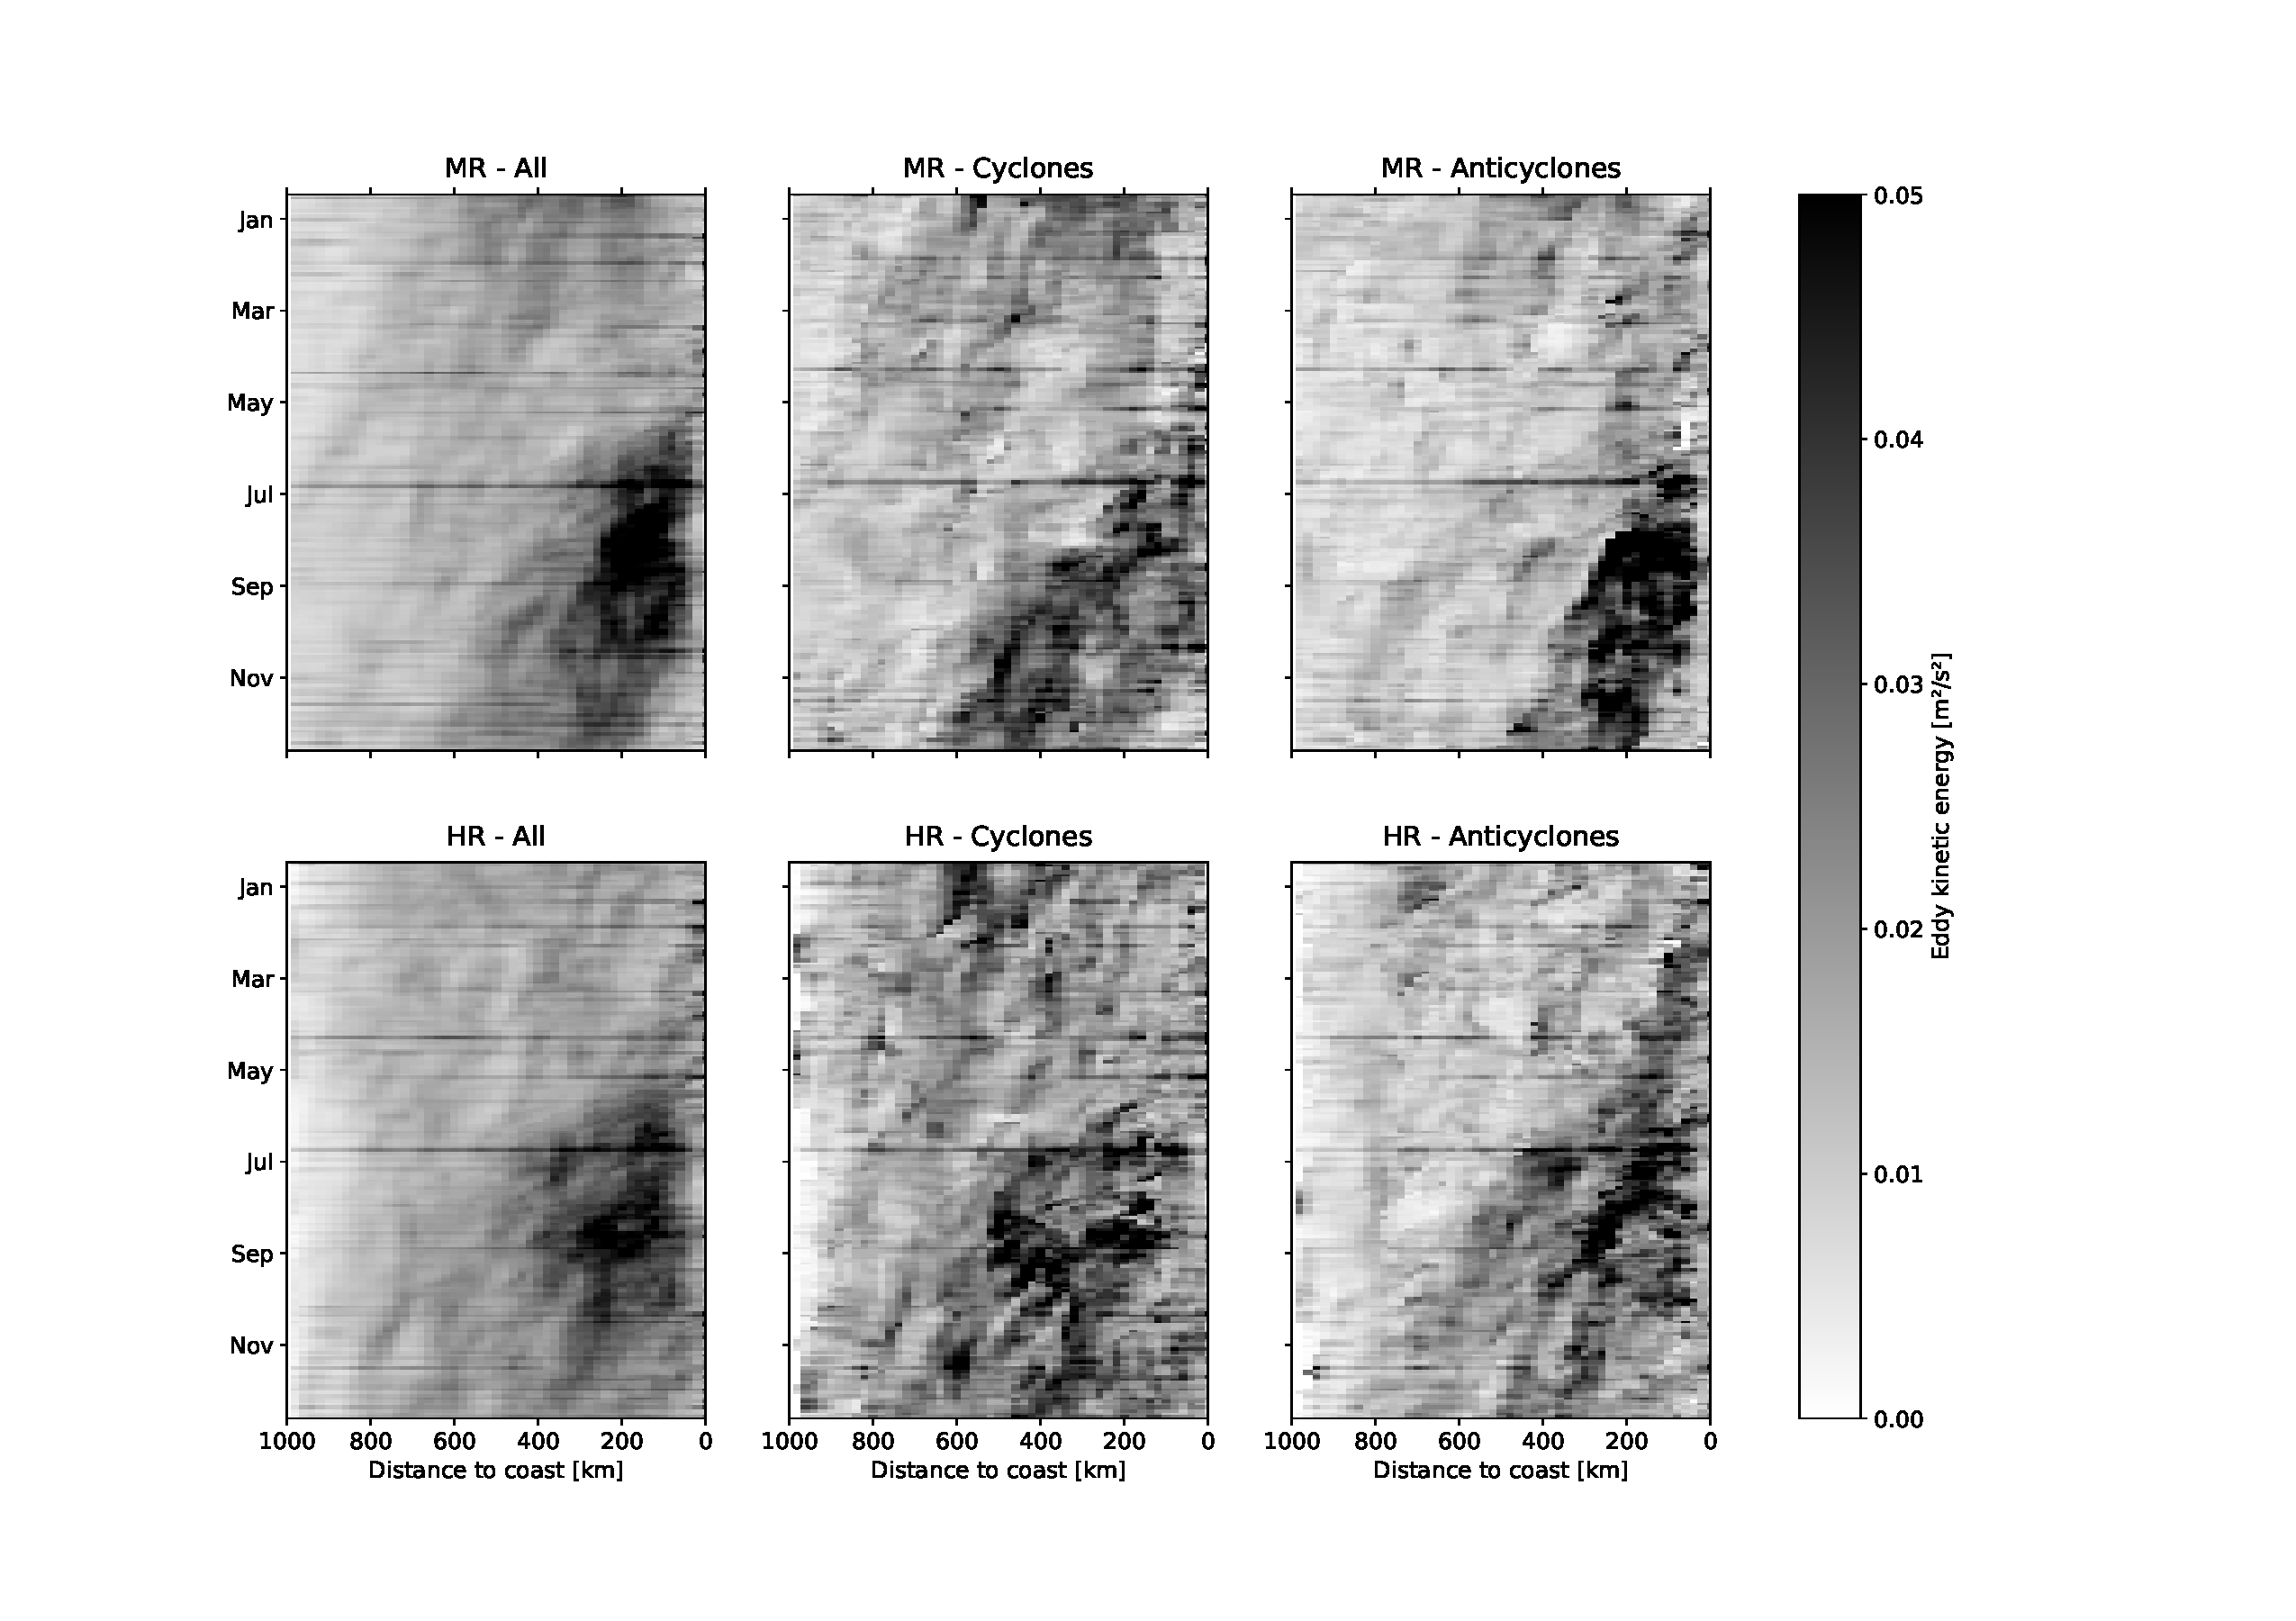
\includegraphics[width=24cm, trim=0 0 0 2cm]{../figures/result_eddies_eke.pdf}
    \vspace*{-2.0cm}\caption[Eddy Kinetic Energy]{\textbf{Eddy Kinetic Energy} of \ac{mr} (top) and \ac{hr} (bottom). The \ac{eke} is shown for the whole domain (i.e. independent of eddy detections) left, for cyclones in the center and for anticyclones right.}
    \label{fig:eddy-eke}
\end{sidewaysfigure}
\\
In the nearshore region, an outstanding difference between \ac{mr} and \ac{hr} is the enhanced activity of eddies in spring (see \autoref{fig:eddy-eke}). From March to June, the mean \ac{eke} of nearshore anticyclones is $\SI[separate-uncertainty]{18.3(4)e-3}{\metre\squared\per\second\squared}$ in \ac{mr} compared to $\SI[separate-uncertainty]{26.2(4)e-3}{\metre\squared\per\second\squared}$ in \ac{hr}. This matches to the increase of overall EKE during spring mentioned above. A reason for the increase could be a difference in the strength of the \ac{cuc}, because the formation of nearshore eddies is strongly driven by vertical shear induced by the undercurrent \autocite{checkley-2009-currentstructure-calcs, kurian-2011-eddy-props}. The strength of the \ac{cuc} can be assessed by the horizontal velocity component $u$ because the curvilinear gridlines of the model are approximately parallel to the coast (see \autoref{sec:data-methods-model}). From February to March, the \ac{cuc} and the \ac{cc} are stronger in \ac{hr} than in \ac{mr} (see \autoref{fig:undercurrent}). In contrast, both currents are of similar strength in \ac{hr} and \ac{mr} from June to August. The stronger \ac{cuc} generates more shear which might be a reason for the enhanced eddy activity in early spring. An investigation of the exact reason for the different strength is out of the scope of this study. Nevertheless, it should be noted that both models differ from observations of \textcite[see their Figure 4.2.3.1 to 4.2.3.4]{rudnick-2017-calcs-climatology} or model results of \textcite[see their Figure 20]{renault-2020-model-descr}. Therefore, future studies should pay special attention to the tuning of the \ac{cuc} strength.\\
\\
Before the density anomaly is examined, the vertical structure of the anomalies in mesoscale eddies is briefly discussed. \autoref{fig:eddy-temp} shows the vertical structure of the temperature anomaly in \ac{mr}. It primarily follows the density anomaly, but \textcite{kurian-2011-eddy-props} only report the temperature anomaly. The anomaly extends down to more than $\SI{500}{\metre}$ and has a maximum $\around \SI{100}{\metre}$. A similar depth of maximum anomaly was found by \textcite[see their Figure 16]{kurian-2011-eddy-props}, though they report weaker anomalies ($\SI{-0.78}{\kelvin}$ and $\SI{0.48}{\kelvin}$ compared to $\around\SI{-1.0}{\kelvin}$ and $\around\SI{1.2}{\kelvin}$ in this study). This can be explained by the different definition of anomaly: \textcite{kurian-2011-eddy-props} approximate the mean state as a spatial average over a box of $85\si{\kilo\metre} \times 85\si{\kilo\metre}$ around the eddy core. Considering the typical eddy size, this removes less of the eddy-induced variability from the mean state than the method applied in this study (see \autoref{sec:data-methods-eddymetrics}).\\
\begin{figure}
    \centering
    \hspace*{1cm}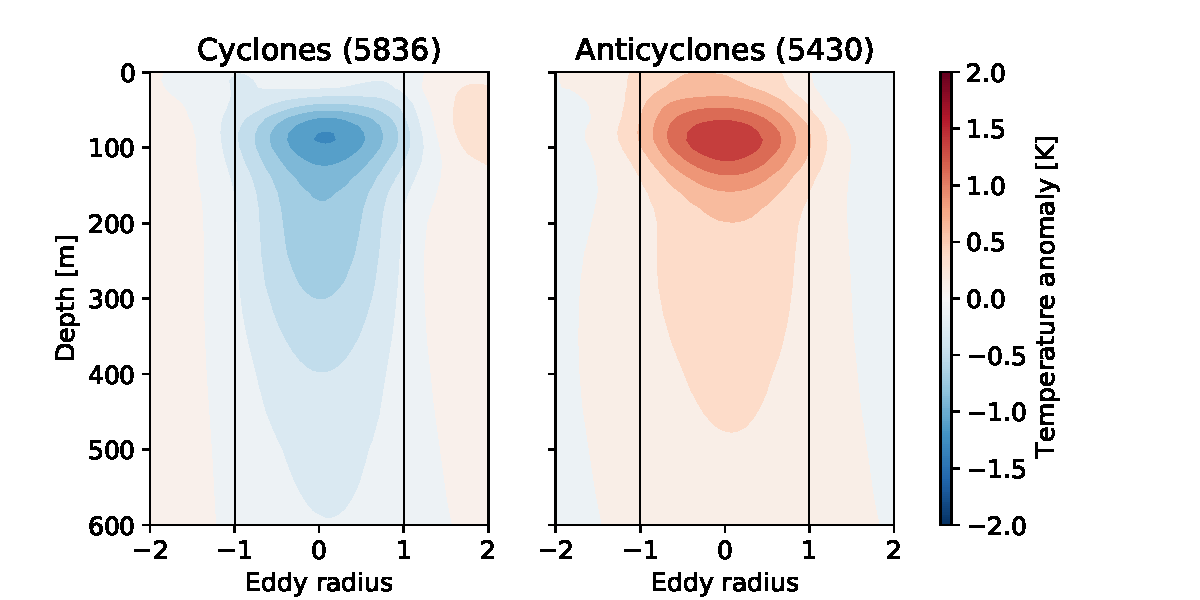
\includegraphics[width=12cm, trim=0 0 1cm 0]{../figures/result_composites_temp.pdf}
    \caption[Vertical structure of temperature anomaly]{\textbf{Vertical structure of temperature anomaly}. The number of aggregated eddies is denoted in brackets.}\label{fig:eddy-temp}
\end{figure}
\\
\\
Regarding the density anomaly, offshore cyclones exhibit a seasonality in \ac{hr} which is not present in \ac{mr}. The average anomaly between $\SI{80}{\metre}$ and $\SI{120}{\metre}$ (which includes the maximum) is shown in \autoref{fig:density-anomaly}. The anomaly in \ac{mr} has little variance (values range from \SIrange{25e-3}{32e-3}{\kilo\gram\per\metre\cubed} without a trend). In contrast, the anomaly in \ac{hr} increases systematically from $\SI{25.4(6)e-3}{\kilo\gram\per\metre\cubed}$ in late winter to $\SI{37.6(6)e-3}{\kilo\gram\per\metre\cubed}$ in late summer.\\
The effect is also visible in \ac{eke} associated with offshore cyclones. \autoref{fig:eddy-eke-comp} shows the relative increase in \ac{eke} from \ac{mr} to \ac{hr}: cyclones start to intensify in late spring and are $\around \SI{50}{\percent}$ more energetic during summer in \ac{hr} than in \ac{mr}. But even during winter the \ac{eke} is $\around \SI{20}{\percent}$ higher in \ac{hr}. This is mainly driven by spontaneous (i.e. not related to eddies coming from nearshore) and localized boosts of the \ac{eke} (see e.g. at $\SI{400}{\kilo\metre}$ off the coast in March, \autoref{fig:eddy-eke}).\\
\begin{figure}
    \centering
    \hspace*{-0.2cm}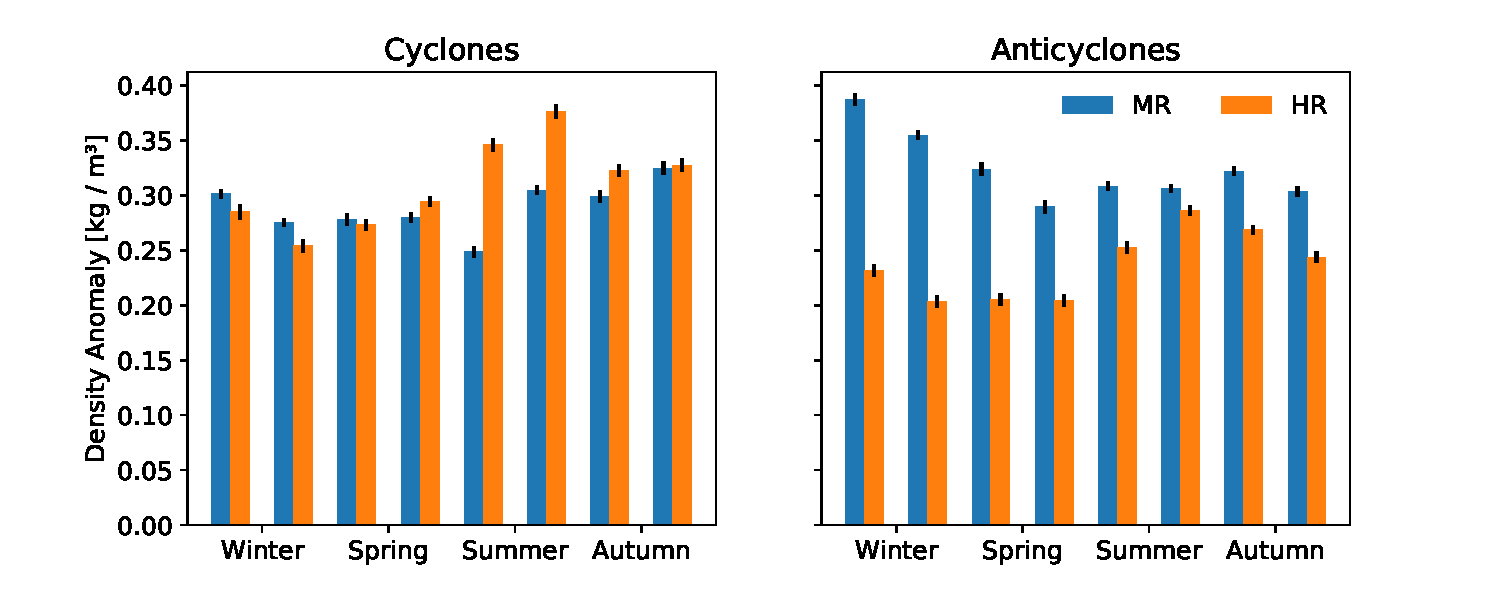
\includegraphics[width=16cm, trim=0 0 0 0]{../figures/result_eddies_density}
    \caption[Offshore density anomaly]{\textbf{Offshore density anomaly}. The black bars denote the interannual variability. Note, that the anomaly is negative in anticyclones.}\label{fig:density-anomaly}
\end{figure}
\begin{figure}
    \centering
    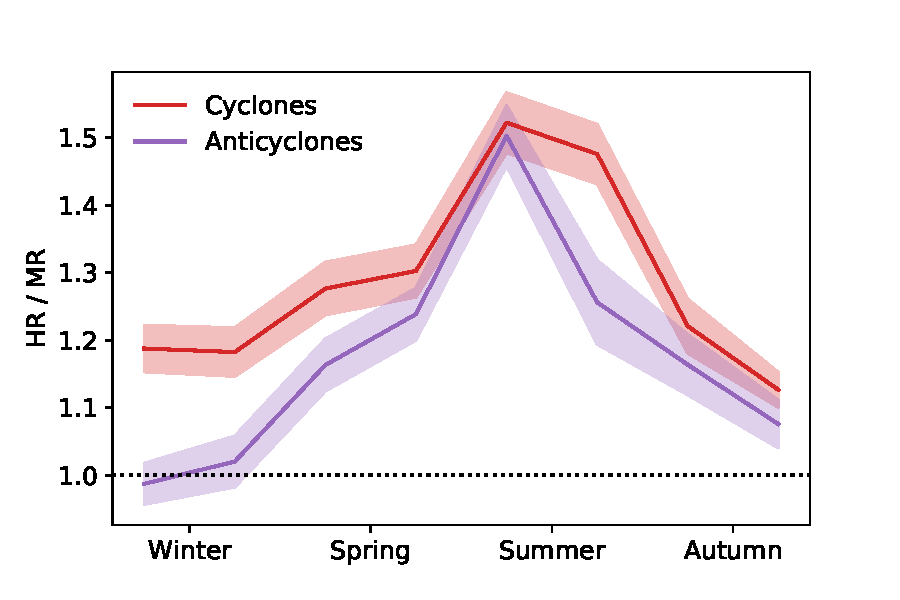
\includegraphics[width=9cm, trim=0 0 0 0]{../figures/result_eddies_eke_comparison}
    \caption[Relative increase in offshore EKE]{\textbf{Relative increase in offshore EKE}. The shaded area represents the interannual variability.}\label{fig:eddy-eke-comp}
\end{figure}
\\
By contrast, the density anomaly of offshore anticyclones differ strongly between \ac{mr} and \ac{hr}. The difference is largest in winter where the anomaly drops from $\SI{-37.1(6)e-3}{\kilo\gram\per\metre\cubed}$ in \ac{mr} to $\SI{-21.8(5)e-3}{\kilo\gram\per\metre\cubed}$ in \ac{hr} (see \autoref{fig:density-anomaly}). This difference is much larger than the maximum difference observed for cyclones. As a result, the year-round density anomaly of anticyclones is smaller than for cyclones in \ac{hr}, whereas it is larger than for cyclones in \ac{mr}. Yet, the seasonality of anticyclones in \ac{hr} is very similar to the seasonality of cyclones. Regarding the \ac{eke} associated with anticyclones, an intensification in late spring and early summer appears which is very similar to cyclones. However, \ac{eke} is hardly increased during winter which is in accordance with the described weakening (see \autoref{fig:eddy-eke-comp}).\\
\\
The presented findings do not depend on the exact choice of the depth range used for averaging the anomaly. This was tested by comparing the presented results for the range \SIrange{80}{120}{\metre} depth to the range \SIrange{25}{200}{\metre} depth. Although the absolute values change, the described trends are still present (see \autoref{fig:density-anomaly2}).\\
\\
In summary, the properties of the detected eddies are consistent with previous studies of the \ac{ccs}, e.g. \textcite{kurian-2011-eddy-props}. The increase in horizontal resolution leads to more smaller eddies ($r_e < \SI{30}{\kilo\metre}$) and impacts the strength of eddies, nearshore and offshore. In the nearshore region, eddy activity is enhanced during spring which is probably related to a stronger \ac{cuc}. In the offshore region, the density anomaly exhibits a seasonality in \ac{hr} with a minimum during winter and a maximum during summer. Compared to \ac{mr}, the anomaly of anticyclones is strongly damped in \ac{hr} during winter and spring. This is accompanied with an increased ratio of cyclones to anticyclones and less stable anticyclonic tracks in \ac{hr}.